\chapter{The TRK Codebase: Additional Algorithms}
\label{cha:code2}
In the previous chapter I examined the basic usage of the TRK statistic to fit models to data, including fitting scale optimization, likelihood maximization, and model parameter probability distribution generation. These features are satisfactory for many fitting tasks, but more complicated situation may arise that require special, generalized treatment. In this chapter, I will first introduce an algorithm developed to remove correlation between model parameters. From here, I will then examine the more complicated, but general case of having asymmetric uncertainties, intrinsic and/or extrinsic, in a dataset, and how this can be fitted to as part of the TRK suite.

\section{Automatic Model Parameter Correlation Removal and Pivot Points}
\label{sec:pivot}
To begin, consider some linear model of the form $y=mx+b$; typically, the best-fit slop $m$ will be correlated with the best-fit intercept $b$, i.e. the confidence ellipse between the two parameters in parameter space will be tilted somewhat. This arises from the implicit choice of setting the intercept of the line at $x=0$; such a choice can create an effect where $m$ depends on the choice of $b$. Described as a ``lever-arm'' effect in \textcite{trotter}, this $x-$intercept choice mathematically corresponds to choosing some \textit{pivot point} $x_p$ for a model defined as $y=m(x-x_p)+b$. Choosing some $x_p$ will affect the best-fit $b$, which can in turn affect the best-fit $m$ to some degree. As shown in \textcite{trotter}, an optimal choice for $x_p$ exists such that the correlation of $b$ and $m$ is minimized (for some dataset).

\begin{figure}
    \centering
    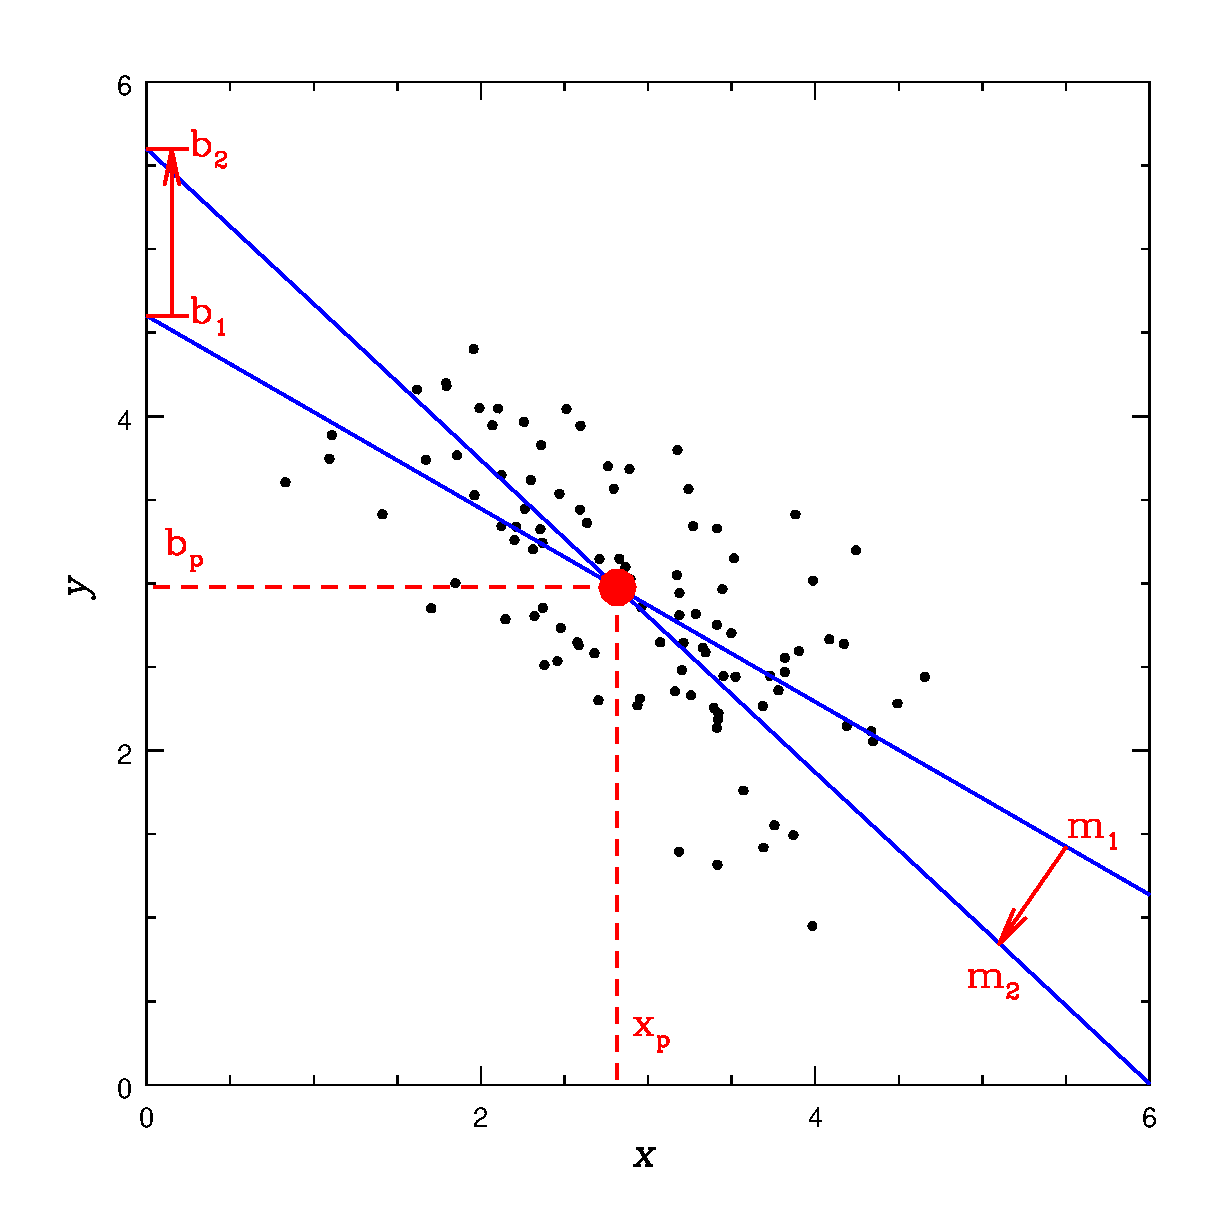
\includegraphics[width=0.8\linewidth]{figures/fig_pivot.eps}
    \caption{From \textcite{trotter}, this figure illustrates how two different choices of pivot point $x_p$ for the linear model $y=m(x-x_p)+b$ results in two different best-fit values for $b$, which in turn correlate to two different best-fit values for $m$. As shown, both of these lines intersect at some optimum pivot point $x_p$, plotted in red; if this optimal $x_p$ is chosen when fitting the model, the correlation between $b$ and $m$ will be minimized.}
    \label{fig:pivotpoint}
\end{figure}

We have devised an algorithm for automatically determining the pivot point for some model; I note that it can be used not just on linear models, but also any linearizable model, as long as the model can be (re-)written in the form of $y=m(x-x_p)+b$. As an example, consider the power-law model $\displaystyle y(x)=a_0\left(\frac{x}{10^{x_p}}\right)^{a_1}$. To linearize this, begin by taking the log of both sides as
\begin{equation}
\begin{split}
    \log_{10}y(x)&=\log_{10}\left[a_0\left(\frac{x}{10^{x_p}}\right)^{a_1}\right]=\log_{10}a_0 + \log_{10}\left(\frac{x}{10^{x_p}}\right)^{a_1}=\log_{10}a_0 + a_1\log_{10}\left(\frac{x}{10^{x_p}}\right)\\&= \log_{10}a_0 + a_1\left[\log_{10}x - \log_{10}10^{x_p}\right] = \log_{10}a_0 + a_1\left(\log_{10}x - x_p\right).
\end{split}
\end{equation}
As such, the linearized version of the power law has intercept $\log_{10}a_0\rightarrow b$, slope $a_1\rightarrow m$, and the data transforms as $\log_{10}y\rightarrow y$ and $\log_{10}x\rightarrow x$.

To introduce our correlation removal/pivot point-finding algorithm, begin by considering two linear (or linearized) fits 
\begin{equation}
\label{eq:2lines}
    y=m_1(x-x_p)+b_1 \qquad\text{and}\qquad y=m_2(x-x_p)+b_2
\end{equation}
with some shared pivot point $x_p$ (see Figure \ref{fig:pivotpoint}). To determine the \textit{optimum} pivot point, I take an iterative approach. As shown in Figure \ref{fig:pivotpoint}, the optimum pivot point should be the $x-$value where the two lines intersect; as such, we set Equations \eqref{eq:2lines} equal to each other and solve to obtain
\begin{equation}
    \label{eq:ppointeqn}
    x=x_p+ \frac{b_1-b_2}{m_2-m_1}.
\end{equation}

In order to use Equation \eqref{eq:ppointeqn} to solve for the optimum pivot point, we need two sets of slop and intercept parameters. However, what parameters should be used? Because no choice is known \textit{a priori},Ie take a Monte Carlo-based approach by using the Metropolis Hastings algorithm (Algorithm \ref{algo:mcmc}) to generate a large sampling (e.g. $R\sim 10,000$) of intercept and slope parameters $(b,m)$, given some previous iteration (or guess, if on the first iteration) of the pivot point $x_p=x_p^\text{old}$. I then generate $K\sim 100,000$ randomly-drawn 2-combinations of pairs of $(b,m)$ from this sample (i.e. various $\{(b_1,m_1),(b_2,m_2)\}$ of Equation \eqref{eq:ppointeqn})\footnote{I note that although I don't use explicit mechanisms to avoid duplicate 2-combinations, there are $\binom{10,000}{2} \simeq 5\times 10^7$ possible randomly-chosen 2-combinations from the set of $10,000$ samples, so if $100,000$ are combinations drawn, there is only a $\simeq 0.2\%$ chance of having a single duplicate.}. From this, I compute $100,000$ possible new pivot points $x_p^\text{new}$ using Equation \eqref{eq:ppointeqn}. From here, how can we use this \textit{distribution} of $x_p^\text{new}$ to determine the optimal $x_p^\text{new}$, i.e. the next iteration of the true optimal pivot point that will minimize correlation?

To start, I desired to choose a weight $w_{x_p^\text{new}}$ for each value of $x_p^\text{new}$ according to the uncertainty $\sigma_{x_p^\text{new}}$ of it's computation, i.e. $w_{x_p^\text{new}}=1/\sigma_{x_p^\text{new}}^2$, given the $\{(b_1,m_1),(b_2,m_2)\}$ that were used to compute it\footnote{This relationship between weight and uncertainty assumes (approximately) Gaussian error.}. To do so, I used standard propagation of uncertainty to first linear order with Equation \eqref{eq:ppointeqn} to obtain
\begin{equation}
\label{eq:ppointweight1}
\sigma_{x_p^\text{new}} \simeq \sqrt{2\left(\frac{\sigma_b}{m_2-m_1}\right)^2 + 2\left[\frac{b_1-b_2}{(m_2-m_1)^2}\right]^2\sigma_m^2}\,,
\end{equation}
where I've assume that the uncertainties $\sigma_{b_1}=\sigma_{b_2}\equiv\sigma_b$ and $\sigma_{m_1}=\sigma_{m_2}\equiv\sigma_m$. Next, note that for a linear model $y=m(x-x_p)+b\equiv mx^\prime+b$, we have that $\sigma_b^2=\sigma_m^2\overline{(x^\prime)^2}=\sigma_m^2\overline{(x-x_p)^2}$, where the overline indicates an average over all $N$ datapoints (\textcite{morrison2014obtaining}). Combining this with Equation \eqref{eq:ppointweight1}, we now have that 
\begin{equation}
\label{eq:ppointweight2}
\sigma_{x_p^\text{new}} \simeq \sqrt{2\frac{\sigma_m^2\overline{(x-x_p)^2}}{(m_2-m_1)^2} + 2\frac{(b_1-b_2)^2}{(m_2-m_1)^4}\sigma_m^2}=\sqrt{2}\sigma_m\sqrt{\frac{\overline{(x-x_p)^2}}{(m_2-m_1)^2} + \frac{(b_1-b_2)^2}{(m_2-m_1)^4}}\,.
\end{equation}

Given that each $x_p^\text{new}$ can be weighted according to $w_{x_p^\text{new}}=1/\sigma_{x_p^\text{new}}^2$, we can factor out constants of proportionality in Equation \eqref{eq:ppointweight2} to obtain
\begin{equation}
w_{x_p^\text{new}} \propto \left[\frac{\overline{(x-x_p)^2}}{(m_2-m_1)^2} + \frac{(b_1-b_2)^2}{(m_2-m_1)^4}\right]^{-1}\,.
\end{equation}
Finally, note that for our iterative approach, $x$ ranges over the sample of the $K=100,000$ new pivot points $x_p^\text{new}$ computed from Equation \eqref{eq:ppointeqn}, and $x_p$ is the previous iteration's optimal single pivot point $x_p^\text{old}$. As such, a single $i^\text{th}$ new pivot point $x_{p,i}^\text{new}$ computed using some $\{(b_1,m_1),(b_2,m_2)\}$ with Equation \eqref{eq:ppointeqn} is weighted according to 
\begin{align}
\label{eq:ppointweight}
w_{x_{p,i}^\text{new}} &\propto\displaystyle \left[\frac{\sum_{j=1}^{K}\left[\left(x_p^\text{old}+ \frac{b_{1,j}-b_{2,j}}{m_{2,j}-m_{1,j}}\right)-x_p^\text{old}\right]^2}{K(m_2-m_1)^2} + \frac{(b_1-b_2)^2}{(m_2-m_1)^4}\right]^{-1} \nonumber \\
&=\displaystyle\left[\frac{\sum_{j=1}^{K}\left(\frac{b_{1,j}-b_{2,j}}{m_{2,j}-m_{1,j}}\right)^2}{K(m_2-m_1)^2} + \frac{(b_1-b_2)^2}{(m_2-m_1)^4}\right]^{-1}\,,
\end{align}
which is the final expression that is used. Finally, I take the weighted half-sample mode (i.e. \textcite{bickel2005fast}) of the $K=100,000$ values for $x_p^\text{new}$ weighted according to Equation \eqref{eq:ppointweight}, and use that as the next iteration for the optimum $x_p$. From here, I iterate until convergence.

\begin{figure}
    \centering
    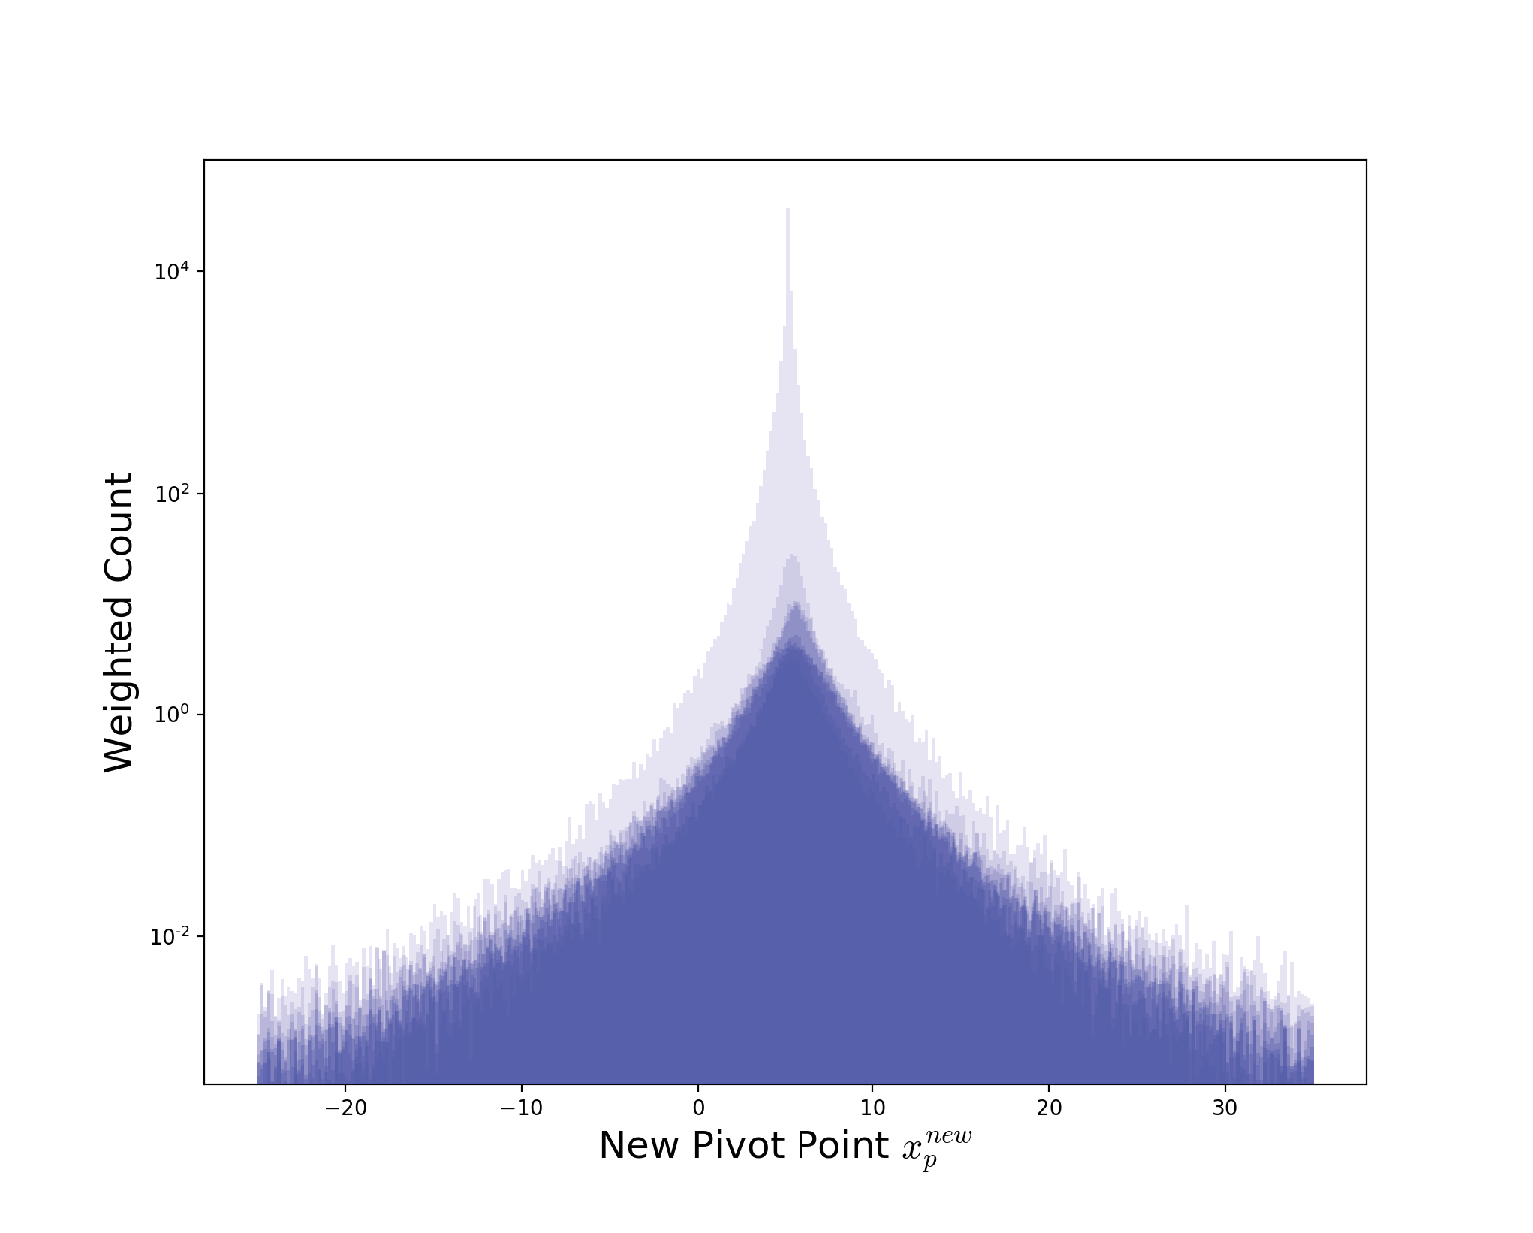
\includegraphics[width=0.8\linewidth]{figures/pivotpointdist.eps}
    \caption{Ten different iterations for the MCMC-generated distributions of new pivot points $x_p^\text{new}$ computed with Equation \eqref{eq:ppointeqn} and weighted according to Equation \eqref{eq:ppointweight}, overlapped. For each iteration we take the optimal value of the new pivot point to be the weighted half-sample mode (see \textcite{bickel2005fast}) of that iteration's distribution, and use this optimal value as $x_p^\text{old}$ for the next iteration in order to compute the next distribution of $x_p^\text{new}$.}
    \label{fig:ppointiters}
\end{figure}

I summarize the pivot point-finding/correlation removal method in Algorithm \ref{algo:pivotpoint}. Once the final pivot point has been found, it is stored as part of the model, and the rest of the TRK algorithm can be used as normal. As an example of this method, in Fig. \ref{fig:linfitnocorr} I show the results of running the pivot point optimization algorithm on the same linear fit dataset as in Figure \ref{fig:linfit} of \S\ref{sec:linfitex}, then running the regular TRK scale optimization, fit and MCMC uncertainty computation as usual. Observe in this figure how the best-fit slope $m$ is mostly unchanged from Figure \ref{fig:linfit}, but the intercept $b$ is noticeably different. Most notably, the parameter space confidence ellipse of $b$ and $m$ is no longer tilted, indicating a loss of correlation between the two parameters. Quantifiably, note that for the fit in Figure \ref{fig:linfit} where the pivot point was not optimized beforehand, the sampled $(b,m)$ has a Pearson correlation coefficient of $R^2 = -0.502$, indicating (negative) correlation as expected. On the other hand, when the pivot point \textit{is} optimized before running this fit, shown in Fig. \ref{fig:linfitnocorr}, the same correlation coefficient is only $R^2=0.056\simeq 0$, indicating almost no correlation, as expected.

\begin{algorithm}
\label{algo:pivotpoint}
\caption{Method to remove model parameter correlation/determine pivot point for linearized models}
\DontPrintSemicolon
    \SetKwInOut{Input}{Input}
    \SetKwInOut{Output}{Output}
    \SetKwProg{Fn}{Function}{}{}
    \Fn{FindPivotPoint}{
        \Input{Linearized model of the form $y_c(x)=m(x-x_p)+b$, dataset $D\equiv\{x_n,y_n,\sigma_{x,n},\sigma_{y,n}\}$, and initial guess for optimum pivot point $x_p^\text{old}$.}
        \Output{Optimum pivot point $x_p$ that minimizes correlation between model parameters $b$ and $m$.}
        \Begin{
        Initialize $R=10,000, K=100,000$ (by default)\;
        \While{$x_p^\text{new}$ not converged}{
            Initialize empty arrays $\mathcal{X}$, $\mathcal{W}$ for new pivot points and their weights, respectively\;
            Generate $R$ samples of $(b,m)\sim MetHastSampler()$(see Algorithm \ref{algo:mcmc})\;
            Store these samples as the set $\mathcal{P}$\;
            \textit{Compute $K$ new pivot points:}\;
            \For{$i=1,2,\cdots,K$}{
                Randomly draw pair $\{(b_1,m_1),(b_2,m_2)\}$. from $\mathcal{P}$\;
                Let $x_{p,i}^\text{new}=x_p^{old} + \frac{b_1-b_2}{m_2-m_1}$\;
                Store $x_{p,i}^\text{new}$ in $\mathcal{X}$\;
            }
            \textit{Weight these $K$ new pivot points:}\;
            \For{$i=1,2,\cdots,K$}{
                Let weight $w_{x_{p,i}^\text{new}} =\displaystyle\left[\frac{\sum_{j=1}^{K}\left(\frac{b_{1,j}-b_{2,j}}{m_{2,j}-m_{1,j}}\right)^2}{K(m_2-m_1)^2} + \frac{(b_1-b_2)^2}{(m_2-m_1)^4}\right]^{-1}$\;
                Store $w_{x_{p,i}^\text{new}}$ in $\mathcal{W}$\;
            }
            Compute optimum $x_p^\text{new}=WeightedHalfSampleMode(\mathcal{X},\mathcal{W})$\;
            $x_p^\text{new}\rightarrow x_p^\text{old}$\;
        }
        }
        \Return{$x_p = x_p^\text{new}$}
    }
\end{algorithm}


\begin{figure}
    \centering
    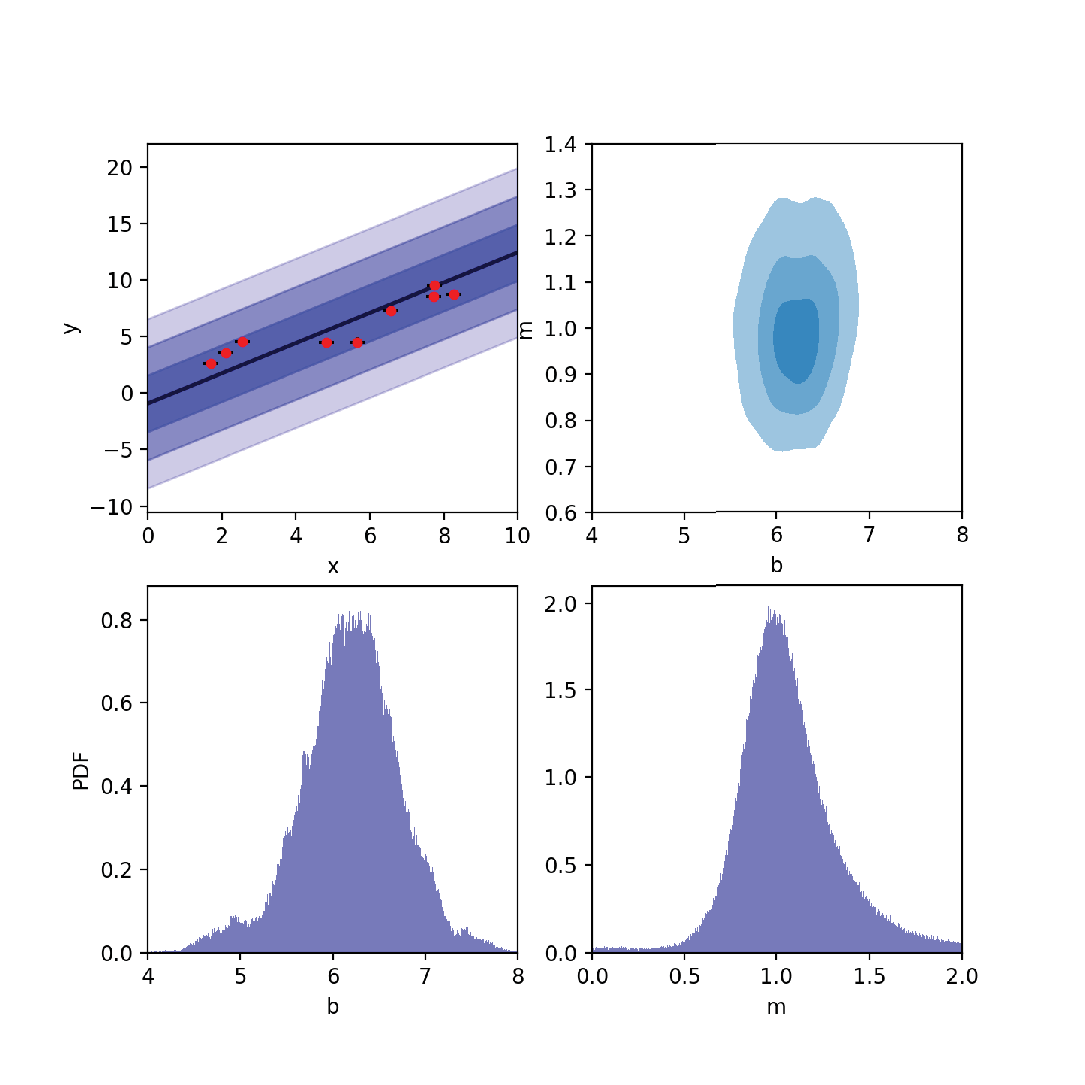
\includegraphics[width=1.0\linewidth]{figures/linfit_sloppy_3shadenoback_pivot.eps}
    \caption{Top left: The same extrinsic scatter-dominated dataset as in Figure \ref{fig:linfit} but now with pivot point $x_p$ in model $y=m(x-x_p)+b$ optimized to minimize correlation between $b$ and $m$, using Algorithm \ref{algo:pivotpoint}. Model is shown with $1-$, $2-$ and $3\sigma$ slop confidence regions visible in blue. Top right: model parameter confidence ellipse with $1-$, $2-$ and $3\sigma$ regions shaded, generated from the posterior probability distributions for $b$ and $m$ found via MCMC, bottom. Note that with pivot point optimized, the confidence ellipse is now no longer tilted as in Fig. \ref{fig:linfit}, indicating the removal of correlation, also evidenced by a Pearson correlation coefficient of $R^2=0.056\simeq 0$.}
    \label{fig:linfitnocorr}
\end{figure}

The ability to minimize parameter correlation for linearized models is a useful and widely applicable addition to the TRK suite. Next, in order to further generalize the TRK statistic, I will explore the possibility of introducing asymmetric error bars and/or slop parameters.

\section{Asymmetric Intrinsic and/or Extrinsic Uncertainty}
\label{sec:asymm}
Throughout this thesis I have only considered models that have intrinsic and extrinsic scatter (i.e. error bars and slop, respectively) that follow \textit{symmetric} Gaussian distributions, i.e. Equation \eqref{eq:symnorm}. However, there remains the distinct possibility for either or both the error bars and the slop/extrinsic scatter to follow \textit{asymmetric} distributions, such as the skew-normal distribution. A number of examples of asymmetric error bars within datasets and/or asymmetric slop within models are given in \textcite{trotter}, and as shown in that work, an excellent approximation of such distributions is defined as the (normalized) \textit{asymmetric} Gaussian distribution,
\begin{equation}
\label{eq:asymnorm}
\mathcal{N}_A(x^\prime;\mu,\sigma_{+},\sigma_-) \equiv \frac{2}{\sqrt{2\pi}(\sigma_{+} +\sigma_{-})} \left\{ \begin{array} {lr}
\exp{\left[-\frac{1}{2}\left(\frac{x^\prime-\mu}{\sigma_{+}}\right)^2\right]}\,\, \mbox{if $x^\prime\geq \mu$} \\
\exp{\left[-\frac{1}{2}\left(\frac{x^\prime-\mu}{\sigma_{-}}\right)^2\right]}\,\, \mbox{if $x^\prime < \mu$} \end{array} \right. \, .
\end{equation}
From here, a 2D asymmetric Gaussian is simply the product of two of these 1D asymmetric Gaussians. Note that this is just a general case of the typical symmetric Gaussian, as this expression simplifies to Equation \eqref{eq:symnorm} when $\sigma_-=\sigma_+\equiv\sigma$.
In the next section, following the work of \textcite{trotter}, I will show how this distribution can be introduced to the TRK statistic in the form of both asymmetric error bars and/or slop.

\subsection{Theory}
I will first introduce some notation. Following \textcite{trotter}, I parameterize the asymmetric $x$ and $y$ error bars of some $n^\text{th}$ datapoint with some parameters $\{\sigma_{x,n+},\sigma_{x,n-}\}$ and $\{\sigma_{y,n+},\sigma_{y,n-}\}$, respectively, following Equation \eqref{eq:asymnorm}. If asymmetric slop/extrinsic scatter along $x$ and/or $y$ is also modeled, such asymmetry is characterize with parameters $\{\sigma_{x+},\sigma_{x-}\}$ and $\{\sigma_{y+},\sigma_{y-}\}$, respectively. Now, in order to perform TRK fits on asymmetric data and/or models, because I have fundamentally generalized the concept of intrinsic and extrinsic scatter, the TRK statistic must be re-developed following the analysis of \S\ref{cha:TRK} with this new asymmetric formalism. To begin, consider a model distribution about the model curve $y_c(x;\vartheta_m)$ that has asymmetric Gaussian slops $(\sigma_{x\pm},\sigma_{y\pm})$, alongside a single $n^\text{th}$ datapoint with asymmetric Gaussian error bars $(\sigma_{x,n\pm},\sigma_{y,n\pm})$, illustrated in Figure \ref{fig:asymm}. Delving into this section, observe that the joint probability of this data-point $p_n$ requires evaluating the convolution of the two asymmetric Gaussians defined by $(\sigma_{x\pm},\sigma_{y\pm})$ and $(\sigma_{x,n\pm},\sigma_{y,n\pm})$, according to Equation \ref{eq:pn}. 

\begin{figure}
    \centering
    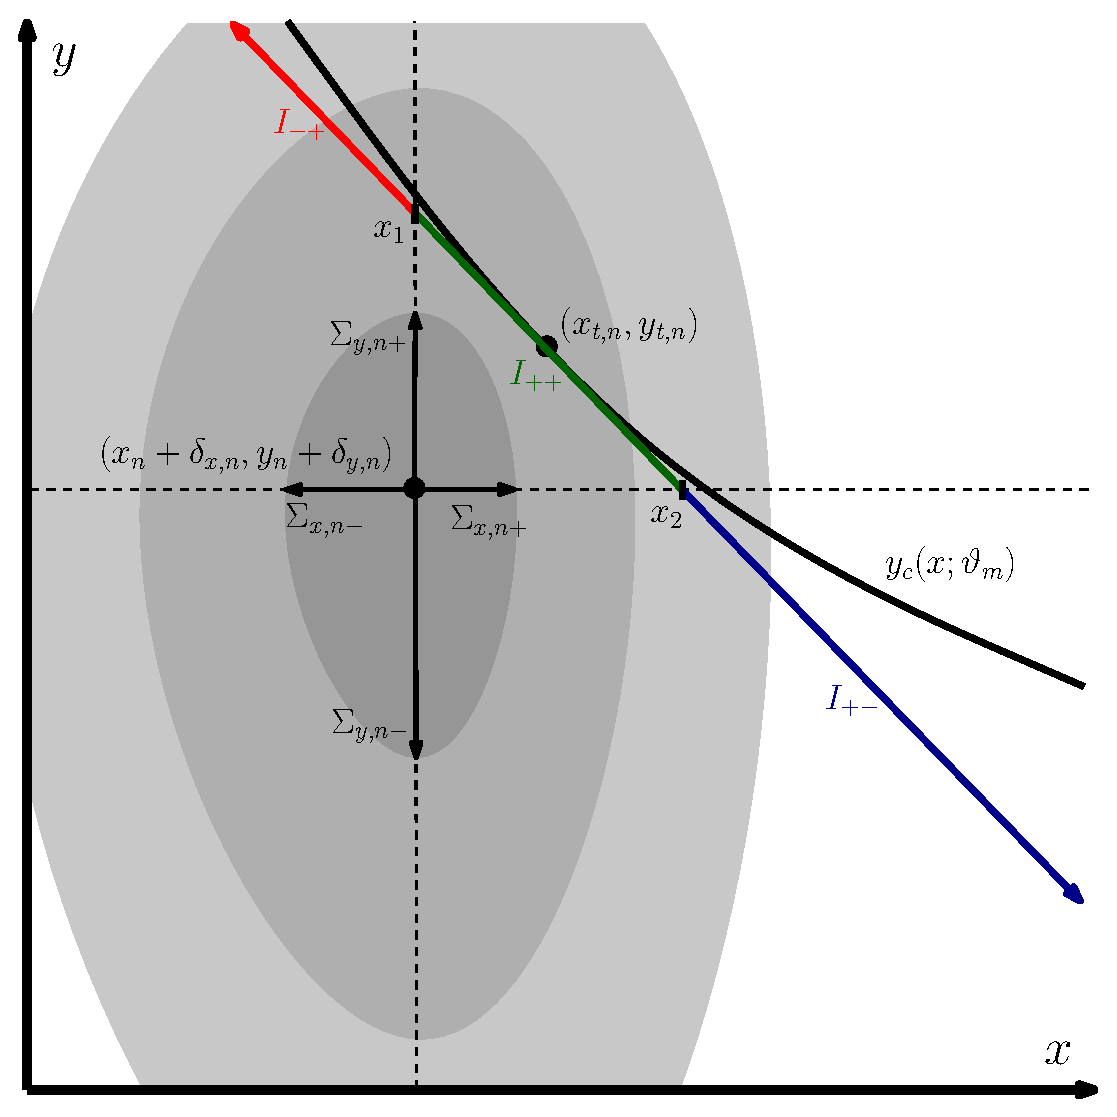
\includegraphics[width=0.8\linewidth]{figures/dia_asymint.eps}
    \caption{From \textcite{trotter}, a visualization of the 2D joint probability for an asymmetric model curve $y_c$ and data-point $(x_n,y_n)$ with asymmetric error bars. This joint probability is an integral that can be approximated by a 2D asymmetric Gaussian with widths $(\Sigma_{x,n\pm}, \Sigma_{y,n\pm})$ centered at some $(x_n+\delta_{x,n}, y_n+\delta_{y,n})$. The integral is broken into three segments according to the quadrants about the convolved centroid $(x_n+\delta_{x,n}, y_n+\delta_{y,n})$, in this case $I_{-+}$, $I_{++}$ and $I_{+-}$, respectively, with subscripts denoting which quadrant the integral/linear approximation of the model curve is located in. For this example, $I_{-+}$ (red) through quadrant 2 has limits $(-\infty,x_1]$, $I_{++}$ (green) through quadrant 1 has limits $[x_1,x_2]$, and $I_{+-}$ (blue) through quadrant 4 has limits $[x_2,\infty)$.}
    \label{fig:asymm}
\end{figure}

As shown in \textcite{trotter}, the convolution of two asymmetric Gaussian distributions does not itself exactly result in an asymmetric Gaussian. However, Trotter showed that an excellent approximation of such a convolution is a 2D asymmetric Gaussian with widths defined by $(\Sigma_{x,n\pm}, \Sigma_{y,n\pm})$ and centroid defined by $(x_n+\delta_{x,n}, y_n+\delta_{y,n})$, where
\begin{align}\label{eq:bigsigsasym}
\Sigma_{x,n\pm} & \equiv \left(\sigma_{x\mp}^2 + \sigma_{x,n\pm}^2\right)^{1/2} \nonumber\\
\Sigma_{y,n\pm} & \equiv \left(\sigma_{y\mp}^2 + \sigma_{x,n\pm}^2\right)^{1/2} \,
\end{align}
and $(\delta_{x,n},\delta_{y,n})$ describes an offset from the data-point which can be found using an empirical method developed by Trotter, given in Algorithm \ref{algo:asymmshifts}, of which the derivation of is beyond the scope of this work. Given that the likelihood is the product of all $N$ of the joint probabilities of the datapoints, using this 2D asymmetric Gaussian approximation for the integral in Equation \eqref{eq:pn} used to compute $p_n$ gives rise to an interesting observation. From \textcite{trotter}, in this asymmetric case the likelihood will have the form of a $\chi^2$-like statistic, but with the datapoint shifted from $(x_n,y_n)$ by $(\delta_{x,n},\delta_{y,n})$, with $\pm1\sigma$ error bars expanded in quadrature by the $\pm$-components of the model slop.

\begin{algorithm}
\label{algo:asymmshifts}
\caption{Method from \textcite{trotter} used to determine offsets $(\delta_{x,n},\delta_{y,n})$ from data-point $(x_n,y_n)$ that are used to compute the 2D asymmetric Gaussian joint probability distribution for some $n^\text{th}$ data-point.}
\DontPrintSemicolon
    \SetKwInOut{Input}{Input}
    \SetKwInOut{Output}{Output}
    \SetKwProg{Fn}{Function}{}{}
    \Fn{GetAsymmShifts}{
        \Input{Asymmetric slop parameters $(\sigma_{x\pm},\sigma_{y\pm})$ and asymmetric error bars $(\sigma_{x,n\pm},\sigma_{y,n\pm})$}
        \Output{Offset $(\delta_{x,n},\delta_{y,n})$}
        \Begin{
        Initialize $\sigma_{L}\equiv\mathrm{max}\left\{\sigma_{y+},\sigma_{y-}\right\}$, $\sigma_{S}\equiv\mathrm{min}\left\{\sigma_{y+},\sigma_{y-}\right\}$,\; $\sigma_{n,L}\equiv\mathrm{max}\left\{\sigma_{y,n+},\sigma_{y,n-}\right\}$,
        $\sigma_{n,S}\equiv\mathrm{min}\left\{\sigma_{y,n+},\sigma_{y,n-}\right\}$, and\; $\sigma_{\mathrm{max}}\equiv\mathrm{max}\left\{\sigma_{L},\sigma_{n,L}\right\}$.\;
        Let $\xi\equiv\frac{\sigma_S}{\sigma_L}+\frac{\sigma_{n,S}}{\sigma_{n,L}}$ and $\eta\equiv \left\{ 
        \begin{array} {lr}
        \frac{\sigma_{n,S}}{\sigma_{n,L}}-\frac{\sigma_{S}}{\sigma_{L}} & \,\,\mbox{if $\sigma_{n,L} < \sigma_{L}$} \, \\
        \frac{\sigma_{S}}{\sigma_{L}}-\frac{\sigma_{n,S}}{\sigma_{n,L}} & \,\,\mbox{if $\sigma_{n,L} \geq \sigma_{L}$} \, .
        \end{array} \right.$\;
        Define $r \equiv \frac{\mathrm{min}\left\{\sigma_{L},\sigma_{n,L}\right\}}{\mathrm{max}\left\{\sigma_{L},\sigma_{n,L}\right\}}$, $\xi^{\prime} = \left\{ \begin{array} {lr}
        \xi & \,\,\mbox{if $\xi\leq 1$}\, \\
        2-\xi & \,\,\mbox{if $\xi > 1$}\, \\
        \end{array} \right.$ and\;
        \vspace{0.3cm}$\eta^{\prime} = \left\{ \begin{array} {lr}
        0 & \,\,\mbox{if $\xi^{\prime} = 0$}\, \\
        2\xi^{\prime}\left[\frac{1}{2}\frac{\eta}{\xi^{\prime}}+1\right]^{n(r)}-\xi^{\prime} & \mbox{otherwise} \,
        \end{array} \right.$, where $n(r) \equiv r^{-0.4087}$.\;
        Compute $\delta_{\ast} = \sigma_{\mathrm{max}}N(r)\left[f(\xi)g(\eta^{\prime})+h(\xi)\right]$, given $N, f, g$ and $h$:\;
        \begin{eqnarray}
        N(r) & = & -0.5326r^2+1.5307r + 0.0019 \\
        f(\xi) & = & \left\{ \begin{array} {lr}
        0 & \,\,\mbox{if $\xi = 0$}\, ,\\
        0.2454\xi^{-1.1452} & \,\,\mbox{if $\xi\leq 1$}\, ,\\
        0.2454\xi^{-0.5203} & \,\,\mbox{if $\xi > 1$} \, ,
        \end{array} \right. \\
        g(\eta^{\prime}) & = & \eta^{\prime 2} \, \\
        h(\xi) & = & -0.042\xi^2-0.1602\xi + 0.4884 \, .
        \end{eqnarray}
        \If{One of the distributions is symmetric}{
            Let $i = \left\{ \begin{array} {lr}
            +1 & \,\,\mbox{if $\sigma_{n,L}=\sigma_{y,n+}$ or $\sigma_L=\sigma_{y-}$} \, \\
            -1 & \,\,\mbox{if $\sigma_{\mathrm{max}}=\sigma_{y,n-}$ or $\sigma_{\mathrm{max}}=\sigma_{y+}$} \,
            \end{array} \right.$\;
            $\delta_{y,n}=i\times\delta_\ast$\;
        }
        \If{Both distributions are asymmetric}{
            Let $i= \left\{ \begin{array} {lr}
            +1 & \,\,\mbox{if $\sigma_{\mathrm{max}}=\sigma_{y,n+}$ or $\sigma_{\mathrm{max}}=\sigma_{y-}$} \, \\
            -1 & \,\,\mbox{if $\sigma_{\mathrm{max}}=\sigma_{y,n-}$ or $\sigma_{\mathrm{max}}=\sigma_{y+}$} \,
            \end{array} \right.$\;
            \If{$\sigma_{L} = \sigma_{y-}$ and $\sigma_{n,L}=\sigma_{y,n+}$, or $\sigma_{L} = \sigma_{y+}$ and $\sigma_{n,L} = \sigma_{y,n-}$}{
                $\delta_{y,n}=i\times\delta_\ast$\;
            }
            \Else{
                $\delta_{y,n} = i\times\delta_{\ast}\times\sin\left(\frac{\pi}{2}\frac{\eta^{\prime}}{\xi^{\prime}}\right)\times\left\{ \begin{array} {lr}
                \xi^{0.7413} & \,\,\mbox{if $\xi \leq 1$} \, \\
                \xi^{-0.1268} & \,\,\mbox{if $\xi > 1$} \,
                \end{array} \right. $\;
            }
        }
        Repeat the above but with $y\rightarrow x$ to compute $\delta_{x,n}$.\;
        \Return{$(\delta_{x,n},\delta_{y,n})$}\;
        }
    }
\end{algorithm}

In order to compute the joint probability $p_n$ for a single datapoint in this asymmetric case, I will first refer back to the example given in Figure \ref{fig:asymm} and follow \S B of \textcite{trotter}. As mentioned, we can approximate the convolution of the two 2D asymmetric Gaussians from Equation \eqref{eq:pn} as a single, shifted 2D asymmetric Gaussian with widths $(\Sigma_{x,n\pm}, \Sigma_{y,n\pm})$ and centroid $(x_n+\delta_{x,n}, y_n+\delta_{y,n})$. Then, following the analysis of \S\ref{sec:2dmodelfitting}, I approximate the model curve $y_c(x;\vartheta_m)$ as a line tangent to the \textit{asymmetric} convolved (and shifted) error ``ellipse'' of the datapoint, such that solving Equation \eqref{eq:tpoint} for the tangent point $x_{t,n}$ requires changing $(\Sigma_{x,n}, \Sigma_{y,n})$ according to which quadrant about the ellipse that the tangent point lies in. For example, if the tangent point is in Quadrant I as in Fig. \ref{fig:asymm}, Equation \eqref{eq:tpoint} transforms with $(\Sigma_{x,n}, \Sigma_{y,n})\rightarrow(\Sigma_{x,n+}, \Sigma_{y,n+})$.\label{pg:tpointasymm}

Observe Equation \eqref{eq:pnanaly}, the symmetric version of the approximate analytic expression for $p_n$, and note the factor $\dv{u_n}{x}$. This factor is dependent on the choice of rotated coordinate system $(u_n,v_n)$, following \S\ref{sec:likelihood}. Combining the choice of $(u_n,v_n)$ that creates the TRK statistic and this asymmetric case, I then find that $\dv{u_n}{x}$ becomes
\begin{equation}\label{eq:dudxasymm}
\dv{u_n}{x}\equiv\left(\dv{u_n}{x}\right)_{\pm\mp} = \frac{m_{t,n}^2\Sigma_{x,n\pm}^2+\Sigma_{y,n\mp}^2}{\sqrt{m_{t,n}^2\Sigma_{x,n\pm}^4+\Sigma_{y,n\mp}^4}} \, ,
\end{equation}
where the subscripts $(\pm\mp)$ are determined by which quadrant the tangent point lines in, i.e $\left(\dv{u_n}{x}\right)_{++}$ corresponds to quadrant I, $\left(\dv{u_n}{x}\right)_{-+}$ to quadrant II, $\left(\dv{u_n}{x}\right)_{--}$ to quadrant III, and $\left(\dv{u_n}{x}\right)_{+-}$ to quadrant IV. In other words, the first subscript indicates the choice of $\Sigma_{x,n\pm}$ and the second indicates the choice of $\Sigma_{y,n\mp}$ in Equation \eqref{eq:dudxasymm}.

Proceeding on, I note that in order to obtain an analytic expression for an asymmetric $p_n$ analogous to Equation \eqref{eq:pnanaly}, we must evaluate the $(-\infty,\infty)$ integral of Equation \eqref{eq:pnappint}. In general, this joint probability integral must now be broken up into three separate integrals $(I_1,I_2,I_3)$, as the tangent line can cross through up to three quadrants of the ellipse, such that $p_n=I_1+I_2+I_3$. Following Figure \ref{fig:asymm}, these three integrals will have limits of $(-\infty, x_1]$, $[x_1,x_2]$ and $[x_2,\infty)$, where $x_1=x_n+\delta_{x,n}$ and $x_2$ is the point where the tangent line intersects with the shifted datapoint centroid, i.e. $y_{t,n}+m_{t,n}(x-x_{t,n})=y_n+\delta_{y,n}$. Note that for all three integrals, the factor $\left(\dv{u_n}{x}\right)_{\pm\mp}$ is the same, given that it only depends on which quadrant the tangent point lies in. Notating the Gaussian cumulative distribution function as
\begin{equation}
\Phi(z)\equiv\int_{-\infty}^z{e^{-\frac{1}{2}x^2}\diff x} \, ,
\end{equation}
evaluating these three integrals with the asymmetric distributions results in the first integral being
\begin{eqnarray}\label{eq:asymmint1}
I_1& = & \left(\dv{u_n}{x}\right)\frac{\kappa\Sigma_{x,n\pm}\Sigma_{y,n\mp}\Phi(z_{-+}(x_1))}{\sqrt{m_{t,n}^2\Sigma_{x,n\pm}^2+\Sigma_{y,n\mp}^2}} \nonumber \\
& &\times \exp\left\{-\frac{1}{2}\left[\frac{y_{t,n}-y_n-\delta_{y,n}-m_{t,n}(x_{t,n}-x_n-\delta_{x,n})}{\sqrt{m_{t,n}^2\Sigma_{x,n\pm}^2+\Sigma_{y,n\mp}^2}}\right]^2\right\} \, 
\end{eqnarray}
with normalization factor\footnote{Note that this normalization factor is the same for all three integrals within any of the four quadrants of the ellipse.} $\kappa\equiv 2/[\pi(\Sigma_{x,n+}+\Sigma_{x,n-})(\Sigma_{y,n+}+\Sigma_{y,n-})]$, where the two sign subscripts of $(\Sigma_{x,n\pm}, \Sigma_{y,n\mp})$, and of the transformed limit of integration
\begin{equation}\label{eq:asymmzlim}
z_{\pm\mp}(x) = \frac{\Sigma_{y,n\mp}^2(x-x_n-\delta_{x,n})+m_{t,n}^2\Sigma_{x,n\pm}^2\left[x-x_{t,n}-(y_n+\delta_{y,n}-y_{t,n})/m_{t,n}\right]}{\Sigma_{x,n\pm}\Sigma_{y,n\mp}\sqrt{m_{t,n}^2\Sigma_{x,n\pm}^2+\Sigma_{y,n\mp}^2}} \,
\end{equation}
are dependent on which two $\Sigma_{x,n\pm}, \Sigma_{y,n\mp}$ widths of the ellipse bound the quadrant that this first integral goes through. For example, in the case of Figure \ref{fig:asymm}, the tangent point is in quadrant I, so this first integral is in quadrant II, which is bounded by $\Sigma_{x,n-}$ and $\Sigma_{y,n+}$, so in this case Equation \eqref{eq:asymmint1} simplifies to
\begin{eqnarray}
I_1& = & \left(\dv{u_n}{x}\right)\frac{\kappa\Sigma_{x,n-}\Sigma_{y,n+}\Phi(z_{-+}(x_1))}{\sqrt{m_{t,n}^2\Sigma_{x,n-}^2+\Sigma_{y,n+}^2}} \nonumber \\
& &\times \exp\left\{-\frac{1}{2}\left[\frac{y_{t,n}-y_n-\delta_{y,n}-m_{t,n}(x_{t,n}-x_n-\delta_{x,n})}{\sqrt{m_{t,n}^2\Sigma_{x,n-}^2+\Sigma_{y,n+}^2}}\right]^2\right\} \, .
\end{eqnarray}
The second integral is similarly found to be
\begin{eqnarray}\label{eq:asymmint2}
I_{2} & = & \left(\dv{u_n}{x}\right)\frac{\kappa\Sigma_{x,n\pm}\Sigma_{y,n\mp}\left[\Phi(z_{\pm\mp}(x_2))-\Phi(z_{\pm\mp}(x_1))\right]}{\sqrt{m_{t,n}^2\Sigma_{x,n\pm}^2+\Sigma_{y,n\mp}^2}} \nonumber \\
& &\times \exp\left\{-\frac{1}{2}\left[\frac{y_{t,n}-y_n-\delta_{y,n}-m_{t,n}(x_{t,n}-x_n-\delta_{x,n})}{\sqrt{m_{t,n}^2\Sigma_{x,n\pm}^2+\Sigma_{y,n\mp}^2}}\right]^2\right\}\,, \nonumber \\
& &  \,
\end{eqnarray}
and the third is found to be
\begin{eqnarray}\label{eq:asymmint3}
I_{3} & = &  \left(\dv{u_n}{x}\right)\frac{\Sigma_{x,n\pm}\Sigma_{y,n\mp}\left[1-\Phi(z_{\pm\mp}(x_2))\right]}{\sqrt{m_{t,n}^2\Sigma_{x,n\pm}^2+\Sigma_{y,n\mp}^2}} \nonumber \\
& &\times \exp\left\{-\frac{1}{2}\left[\frac{y_{t,n}-y_n-\delta_{y,n}-m_{t,n}(x_{t,n}-x_n-\delta_{x,n})}{\sqrt{m_{t,n}^2\Sigma_{x,n\pm}^2+\Sigma_{y,n\mp}^2}}\right]^2\right\} \,,
\end{eqnarray}
where again, the sign subscripts of $(\Sigma_{x,n\pm}, \Sigma_{y,n\mp})$ and $z_{\pm\mp}(x)$ are dependent on which two $\Sigma_{x,n\pm}, \Sigma_{y,n\mp}$ widths of the ellipse bound the quadrant that the respective integral goes through. Then, continuing with the example in Figure \ref{fig:asymm}, the second integral is in Quadrant I while the third is in Quadrant IV, so we have that
\begin{eqnarray}
I_{2} & = & \left(\dv{u_n}{x}\right)\frac{\kappa\Sigma_{x,n+}\Sigma_{y,n+}\left[\Phi(z_{++}(x_2))-\Phi(z_{++}(x_1))\right]}{\sqrt{m_{t,n}^2\Sigma_{x,n+}^2+\Sigma_{y,n+}^2}} \nonumber \\
& &\times \exp\left\{-\frac{1}{2}\left[\frac{y_{t,n}-y_n-\delta_{y,n}-m_{t,n}(x_{t,n}-x_n-\delta_{x,n})}{\sqrt{m_{t,n}^2\Sigma_{x,n+}^2+\Sigma_{y,n+}^2}}\right]^2\right\}\,, \nonumber \\
& &  \,
\end{eqnarray}
and
\begin{eqnarray}
I_{3} & = &  \left(\dv{u_n}{x}\right)\frac{\Sigma_{x,n+}\Sigma_{y,n-}\left[1-\Phi(z_{+-}(x_2))\right]}{\sqrt{m_{t,n}^2\Sigma_{x,n+}^2+\Sigma_{y,n-}^2}} \nonumber \\
& &\times \exp\left\{-\frac{1}{2}\left[\frac{y_{t,n}-y_n-\delta_{y,n}-m_{t,n}(x_{t,n}-x_n-\delta_{x,n})}{\sqrt{m_{t,n}^2\Sigma_{x,n+}^2+\Sigma_{y,n-}^2}}\right]^2\right\} \,.
\end{eqnarray}
From here, the joint probability of the datapoint is found with $p_n=I_1+I_2+I_3$, which is used to define the TRK statistic (i.e. the likelihood) in the same way as the symmetric case.

\subsection{Implementation}
The introduction of asymmetric error bars and/or slop to the TRK suite manifests in a number of ways, the first being the change in the TRK likelihood function $\mathcal{L}^\text{TRK}$.
I have shown how to compute the joint probability $p_n$ for a single $n^\text{th}$ data-point with asymmetric error bars and/or slop, by adding up the three integrals $I_1$, $I_2$ and $I_3$ of Equations \eqref{eq:asymmint1}, \eqref{eq:asymmint2} and \eqref{eq:asymmint3}, respectively. From here, $\mathcal{L}^\text{TRK}$ is simply the product of all $N$ of the $p_n$ of the datapoints, following Equation \eqref{eq:likelibasic}. An essential, but not necessarily obvious thing to point out is that now, there are (up to) \textit{four} slop parameters in total, $(\sigma_{x+}, \sigma_{x-}, \sigma_{y+}, \sigma_{y-})\equiv(\sigma_{x\pm}, \sigma_{y\pm})$. As such, maximizing $\mathcal{L}^\text{TRK}$/ minimizing $-2\ln\mathcal{L}^\text{TRK}$ to find a best fit with the Nelder-Mead method as described in \S\ref{sec:simplex} will now require performing the optimization with respect to all $M+4$ parameters, given $M$ non-slop model parameters. Furthermore, as discussed on page \pageref{pg:tpointasymm}, the driving equation of the tangent point-finding routine, Equation \eqref{eq:tpoint}, must be evaluted with the correct two $(\Sigma_{x,n\pm},\Sigma_{y,n\pm})$, according to which quadrant of the datapoint ellipse the tangent point is located in. I also note that the \textit{shifted} data-point centroid $(x_n+\delta_{x,n}, y_n+\delta_{y,n})$, found with Algorithm \ref{algo:asymmshifts}, must be used in place of the unshifted $(x_n,y_n)$ of the symmetric case at all steps of running a TRK fit. Finally, I note that the scale optimization procedure of \S\ref{sec:scaleop} does not obviously generalize for the asymmetric case; this issue will be tackled in the future, as discussed in \S\ref{cha:future}.